%Gerado automaticamente por mathcha.io
%Obrigado por existir, mathcha.io. Um dia te pago um pastel

\tikzset{every picture/.style={line width=0.75pt}} %set default line width to 0.75pt        

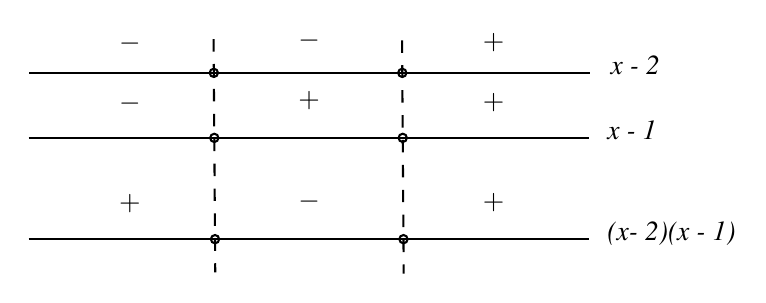
\begin{tikzpicture}[x=0.75pt,y=0.75pt,yscale=-1,xscale=1]
%uncomment if require: \path (0,300); %set diagram left start at 0, and has height of 300

%Straight Lines [id:da6190276703964156] 
\draw    (160.6,109.67) -- (430.6,109.67) ;
%Straight Lines [id:da9836177427755605] 
\draw    (160.33,141) -- (430.33,141) ;
%Straight Lines [id:da8096639673115349] 
\draw    (160.33,189.8) -- (430.33,189.8) ;
%Straight Lines [id:da2202505370108293] 
\draw  [dash pattern={on 4.5pt off 4.5pt}]  (249.4,93.4) -- (250.2,205.8) ;
%Straight Lines [id:da12354861824101204] 
\draw  [dash pattern={on 4.5pt off 4.5pt}]  (340.2,94) -- (341,206.4) ;

% Text Node
\draw (202.4,89.6) node [anchor=north west][inner sep=0.75pt]    {$-$};
% Text Node
\draw (202.4,118.4) node [anchor=north west][inner sep=0.75pt]    {$-$};
% Text Node
\draw (288.8,88.4) node [anchor=north west][inner sep=0.75pt]    {$-$};
% Text Node
\draw (288.8,117.2) node [anchor=north west][inner sep=0.75pt]    {$+$};
% Text Node
\draw (377.6,89.2) node [anchor=north west][inner sep=0.75pt]    {$+$};
% Text Node
\draw (377.6,118) node [anchor=north west][inner sep=0.75pt]    {$+$};
% Text Node
\draw (202.4,166.8) node [anchor=north west][inner sep=0.75pt]    {$+$};
% Text Node
\draw (288.8,165.6) node [anchor=north west][inner sep=0.75pt]    {$-$};
% Text Node
\draw (377.6,166.4) node [anchor=north west][inner sep=0.75pt]    {$+$};
% Text Node
\draw (439.2,100.2) node [anchor=north west][inner sep=0.75pt]   [align=left] {{\fontfamily{ptm}\selectfont \textit{x - 2}}};
% Text Node
\draw (437.6,131.4) node [anchor=north west][inner sep=0.75pt]   [align=left] {{\fontfamily{ptm}\selectfont \textit{x - 1}}};
% Text Node
\draw (437.6,180.2) node [anchor=north west][inner sep=0.75pt]   [align=left] {{\fontfamily{ptm}\selectfont \textit{(x- 2)(x - 1)}}};

\draw   (340.31, 109.67) circle [x radius= 2, y radius= 2]   ;
\draw   (340.53, 141) circle [x radius= 2, y radius= 2]   ;
\draw   (340.88, 189.8) circle [x radius= 2, y radius= 2]   ;
\draw   (249.52, 109.67) circle [x radius= 2, y radius= 2]   ;
\draw   (249.74, 141) circle [x radius= 2, y radius= 2]   ;
\draw   (250.09, 189.8) circle [x radius= 2, y radius= 2]   ;
\end{tikzpicture}
